\subsection{Evaluation Datasets}

We evaluated our experiments on six datasets. \textbf{SST2} \cite{socher-etal-2013-recursive} \textbf{SST5} \cite{socher-etal-2013-recursive}, \textbf{MR} \cite{10.3115/1219840.1219855} and \textbf{Subj} \cite{10.3115/1218955.1218990} are four datasets for sentiment classification; \textbf{AGNews} \cite{NIPS2015_250cf8b5} is a topic classification dataset; and \textbf{CB} \cite{Marneffe2019TheCI} is used
for natural language inference.

\subsection{Evaluation Metrics}

In the following sections we describe the evaluation metrics used to compare the behavior of ICL and finetuning.
To ensure an optimal comparison, we have adopted the identical metrics as introduced in \cite{dai2023gpt}:
We design three metrics to measure the similarity between ICL and finetuning at three different levels: the prediction level, the representation level, and the attention behavior level. 

% \paragraph{Prediction Recall}

% From the perspective of model prediction, models with similar behavior should have aligned predictions.
% We measure the recall of correct ICL predictions to correct finetuning predictions.
% Given a set of test examples, we count the subsets of examples correctly predicted by each model: $C_{\text{ZSL}}, C_{\text{ICL}}, C_{\text{FT}}$.
% To compare the update each method induces to the model's prediction we subtract correct predictions made in the ZSL setting.
% Finally we compute the \textbf{Rec2FTP} score as: $\frac{ \sizeof{ \left( C_{\text{ICL}} \cap C_{\text{FT}} \right) \setminus C_{\text{ZSL}} } }{ \sizeof{ C_{\text{FT}} \setminus C_{\text{ZSL}} } }$ .
% A higher Rec2FTP score suggests that ICL covers more correct behavior of finetuning from the perspective of the model prediction.

%This measure is agnostic to the inner workings of the attention mechanism.

\paragraph{Attention Output Direction}
In the context of an attention layer's hidden state representation space within a model, we analyze the modifications made to the attention output representation (\textbf{SimAOU}).

For a given query example, let $h^{(l)}_X$ represent the normalized output representation of the last token at the $l$-th attention layer within setting $X$. The alterations introduced by ICL and finetuning in comparison to ZSL are denoted as $h^{(l)}_{ICL} - h^{(l)}_{ZSL}$ and $h^{(l)}{FT} - h^{(l)}_{ZSL}$, respectively. We calculate the cosine similarity between these two modifications to obtain SimAOU ($\Delta FT$) at the $l$-th layer. A higher SimAOU ($\Delta FT$) indicates that ICL is more inclined to adjust the attention output in the same direction as finetuning.
For the sake of comparison, we also compute a baseline metric known as SimAOU (Random $\Delta$), which measures the similarity between ICL updates and updates generated randomly.

\paragraph{Attention Map Similarity}
We use SimAM to measure the similarity between attention maps and query tokens for ICL and finetuning.
For a query example, let $m^{(l,h)}_X$ represent the attention weights before softmax in the $h$-th head of the $l$-th layer for setting $X$. In ICL, we focus solely on query token attention weights, excluding demonstration tokens. Initially, before finetuning, we compute the cosine similarity between $m^{(l,h)}_{ICL}$ and $m^{(l,h)}_{ZSL}$, averaging it across attention heads to obtain SimAM (Before Finetuning) for each layer.
Similarly, after finetuning, we calculate the cosine similarity between $m^{(l,h)}_{ICL}$ and $m^{(l,h)}_{FT}$ to obtain SimAM (After FT). A higher SimAM (After FT) relative to SimAM (Before FT) indicates that ICL's attention behavior aligns more with a finetuned model than a non-finetuned one.


\subsection{Prediction Alignment}
In this section we focus on the perspective of model predictions, regarding both ICL and finetuning as black-box updates to the original zero-shot prediction.
While this analysis provides less insight into the inner workings of ICL, prediction alignment is easily interpretable and seems necessary for downstream applications of such comparisons.

Revisiting the results of \cite{dai2023gpt}, the authors find that find that ICL achieves high \textbf{Rec2FTP} scores across multiple tasks, which means it covers most of the correct predictions of finetuning. 
However their results show a discrepancy between the accuracy of the finetuned model and the ICL setting, average difference of $\textbf{19.38\%}$ relative to the original zero-shot accuracy (Table \ref{acc_rpa}).
%relative diff in acc by task (1_3B)[0.2666666666666666, 0.13994910941475827, 0.24279210925644915, 0.16804407713498629, 0.30021598272138245, 0.045333333333333406]$%
We argue that \textbf{Rec2FTP} is insufficient to quantify prediction alignment in this setting because:
(1) it does not the difference between the number of changes induced by each method;
(2) it does not account for incorrect prediction changes.
Figure \ref{fig:prediction_alignment} shows the number of prediction updates induced by each method.
We measure both changes that result in correct and incorrect predictions.
The results show that overall ICL is more inclided to change the ZSL prediction.
Another noticable trend is that although ICL covers almost all FT correct prediction changes (high Rec2FTP), there are many incorrect prediction updates unique both to FT and to ICL.
This observation shows the importance of measuring incorrect prediction changes as well.

\begin{figure*}[h!]
  \centering
  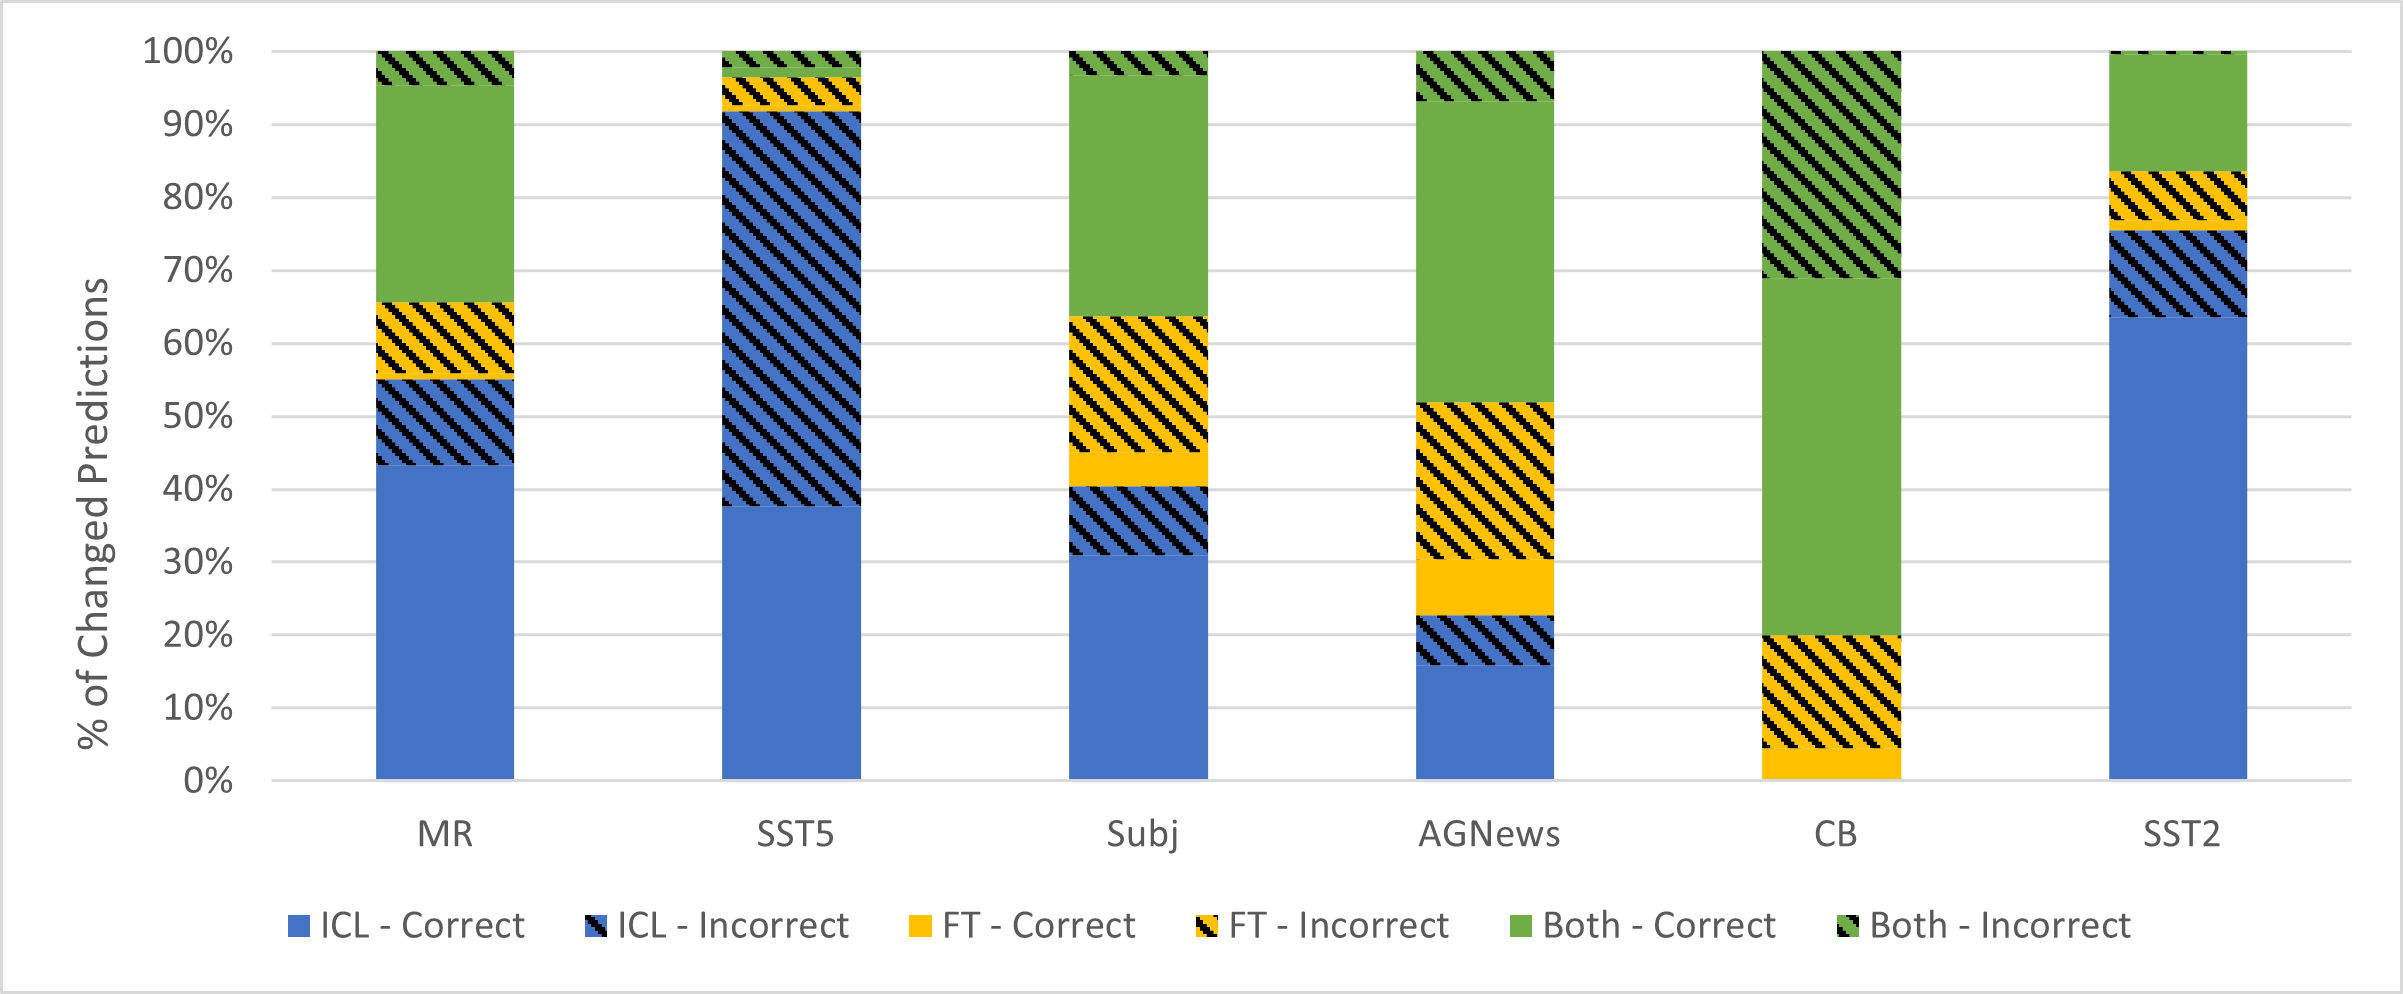
\includegraphics[width=0.98\linewidth,height=6cm]{resources/images/prediction_alignment.png}
  \caption{
    Partition of prediction changes with regards to the zero-shot setting induced by ICL and FT.
    For each task, we evaluate both methods on the same validation set.
    Correct changes are examples that are misclassified in the ZSL setting and are correctly classified following the prediction update.
    incorrect changes are examples whose prediction is changed from the ZSL setting into an incorrect label.
  }
  \label{fig:prediction_alignment}
\end{figure*}

We propose a metric that respects these factors: \textbf{relative prediction alignment} (RPA) to quantify prediction alignment in this setting.
Given a validation set, we denote the subset of example whose prediction is changed with regards to the zero-shot setting by ICL or FT by $D_\text{ICL}$ and $D_\text{FT}$ respectively.
We define the RPA of these updates by: 
\begin{equation*}
  \text{RPA}_{D_\text{ICL}, D_\text{FT}} = \frac{\sizeof{D_\text{ICL} \cap D_\text{FT}}}{\sizeof{D_\text{ICL}} + \sizeof{D_\text{FT}} - \sizeof{D_\text{ICL} \cap D_\text{FT}}} 
\end{equation*}

\begin{table*}[ht!]
  \centering
  \setlength{\tabcolsep}{7pt}
  \begin{tabular}{l | c c c c c c}
  \toprule
  & \textbf{CB} & \textbf{SST2} & \textbf{SST5} & \textbf{Subj} & \textbf{MR} & \textbf{AGNews} \\ 
  \midrule
   ZSL Accuracy & 37.5 & 70.5 & 39.3 & 72.6 & 65.9 & 46.2 \\
   FT Accuracy & 57.1 & 74 & 39.4 & 77.8 & 72.6 & 66.7 \\
   ICL Accuracy & 50 & 92.7 & 45.0 & 90.0 & 89.1 & 79.2 \\
  \midrule
  RPA (\%)           & 80.0 & 16.4 & 3.4 & 36.2 & 34.0 & 48.0 \\
  RPA - Correct (\%) & 91.7 & 19.8 & 3.2 & 48.0 & 40.2 & 63.5 \\
  RPA - Incorrect (\%) & 66.7 & 1.8 & 3.5 & 10.2 & 17.7 & 19.2 \\
  \end{tabular}
  \caption{Validation accuracy and RPA scores for ZSL, finetuning, and ICL settings on all six classification datasets.}
  \label{tab:acc_rpa}
\end{table*}

We report the RPA scores across all tasks in table \ref{tab:acc_rpa}.
For each we also compute the RPA scores computed over only for prediction changes to correct labels, and those for incorrect labels.
The results show that correct prediction changes are more aligned between the two methods.